
\documentclass[
    % -- opções da classe memoir --
    12pt,               % tamanho da fonte
    openright,          % capítulos começam em páginas ímpar
    twoside,            % para impressão em verso e anverso. Oposto a oneside
    a4paper,            % tamanho do papel. 
    % -- opções da classe abntex2 --
    %chapter=TITLE,     % títulos de capítulos convertidos em letras maiúsculas
    %section=TITLE,     % títulos de seções convertidos em letras maiúsculas
    %subsection=TITLE,  % títulos de subseções convertidos em letras maiúsculas
    %subsubsection=TITLE,% títulos de subsubseções convertidos em letras maiúsculas
    % -- opções do pacote babel --
    brazil              % o último idioma é o principal do documento
    ]{abntex2}

% ---
% Pacotes básicos 
% ---
\usepackage{palatino}           % Usa a fonte Latin Modern
\usepackage[T1]{fontenc}        % Selecao de codigos de fonte.
\usepackage[utf8]{inputenc}     % Codificacao do documento (conversão automática dos acentos)
\usepackage{lastpage}           % Usado pela Ficha catalográfica
\usepackage{indentfirst}        % Indenta o primeiro parágrafo de cada seção.
\usepackage{color}              % Controle das cores
\usepackage{graphicx}           % Inclusão de gráficos
\usepackage{microtype}          % para melhorias de justificação
\usepackage{graphicx}
\graphicspath{ {images/} }
% ---
        
% ---
% Informações de dados para CAPA e FOLHA DE ROSTO
% ---
\titulo{Definição do Projeto de Interação Humano-Computador}
\autor{
    Eric Bueno Gauch
    \and
    Bruno Estima Correia Milanesi Castanheira de Souza
    \and
    Filippi Luigi Di Pipi
    \and
    Guilherme Gatto Gonçalves da Silva}
\local{Brasil}
\data{2017, v-1.0.0}
\instituicao{%
  Universidade Presbiteriana Mackenzie -- UPM
  \par
  Faculdade de Computação e Informática
  \par
  Programa de Graduação em Ciência da Computação}
\tipotrabalho{Trabalho Acadêmico}
% O preambulo deve conter o tipo do trabalho, o objetivo, 
% o nome da instituição e a área de concentração 
\preambulo{Definição do projeto da disciplina de Interação Humano-Computador}
% ---

% ---
% Configurações de aparência do PDF final

% alterando o aspecto da cor azul
\definecolor{blue}{RGB}{41,5,195}

% informações do PDF
\makeatletter
\hypersetup{
        %pagebackref=true,
        pdftitle={\@title}, 
        pdfauthor={\@author},
        pdfsubject={\imprimirpreambulo},
        pdfcreator={LaTeX with abnTeX2},
        pdfkeywords={abnt}{latex}{abntex}{abntex2}{trabalho acadêmico}, 
        colorlinks=true,            % false: boxed links; true: colored links
        linkcolor=black,             % color of internal links
        citecolor=blue,             % color of links to bibliography
        filecolor=magenta,              % color of file links
        urlcolor=blue,
        bookmarksdepth=4
}
\makeatother
% --- 

% O tamanho do parágrafo é dado por:
\setlength{\parindent}{1.3cm}

% Controle do espaçamento entre um parágrafo e outro:
\setlength{\parskip}{0.2cm}  % tente também \onelineskip

% ---
% compila o indice
% ---
\makeindex
% ---

% ----
% Início do documento
% ----
\begin{document}

% Retira espaço extra obsoleto entre as frases.
\frenchspacing 

% ----------------------------------------------------------
% ELEMENTOS PRÉ-TEXTUAIS
% ----------------------------------------------------------
% \pretextual

% ---
% Capa
% ---
\imprimircapa
% ---

% ---
% Folha de rosto
% (o * indica que haverá a ficha bibliográfica)
% ---
\imprimirfolhaderosto*
% ---

% ---
% inserir o sumario
% ---
\clearpage
\pdfbookmark[0]{\contentsname}{toc}
\tableofcontents*
\cleardoublepage
% ---

% ----------------------------------------------------------
% ELEMENTOS TEXTUAIS
% ----------------------------------------------------------
\textual

% ----------------------------------------------------------
% CAPÍTULO
% ----------------------------------------------------------
\chapter{Integrantes do Grupo}
% ----------------------------------------------------------

\begin{center}
\begin{tabular}{ | l | l | l | p{5cm} |}
\hline
NOME & TIA \\ \hline
Bruno Estima Correia Milanesi Castanheira de Souza
& 4152272-9 \\ \hline
Eric Bueno Gauch & 4151051-8 \\ \hline
Filippi Luigi Di Pipi & 3143893-8 \\ \hline
Guilherme Gatto Gonçalves da Silva & 4150246-9 \\ \hline
\end{tabular}
\end{center}

% ----------------------------------------------------------
% CAPÍTULO
% ----------------------------------------------------------
\chapter{Assunto a ser Coberto}
% ----------------------------------------------------------





% ----------------------------------------------------------
% CAPÍTULO
% ----------------------------------------------------------
\chapter{Ideia}
% ----------------------------------------------------------






% ----------------------------------------------------------
% CAPÍTULO
% ----------------------------------------------------------
\chapter{Requisitos Funcionais e Não Funcionais}
% ----------------------------------------------------------






% ----------------------------------------------------------
% CAPÍTULO
% ----------------------------------------------------------
\chapter{\textit{Storyboard}}
% ----------------------------------------------------------

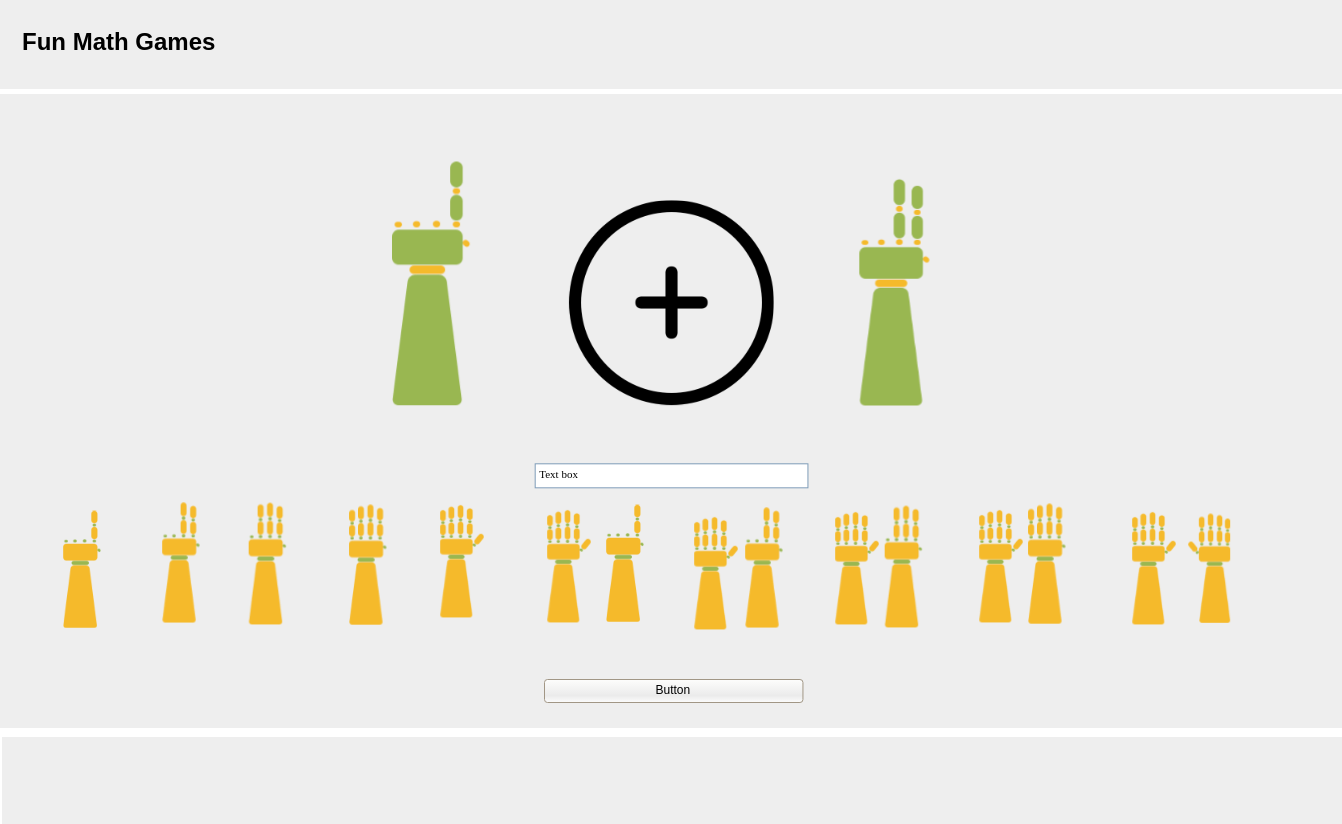
\includegraphics[scale=0.3]{storyboard}

\end{document}
